\documentclass[11pt,a4 paper]{article}
\usepackage{amsmath, amsthm} 
\usepackage[english]{babel}
\usepackage[T1]{fontenc}
\usepackage[utf8]{inputenc}
\usepackage[margin=2cm]{geometry}
\usepackage{indentfirst}
\usepackage{graphicx}
\usepackage{subfigure}
\usepackage{caption}
\usepackage{siunitx}
\captionsetup{tableposition=top,font=small,width=0.8\textwidth}
\usepackage{booktabs}
\usepackage[arrowdel]{physics}
\usepackage{mathtools}
\usepackage{tablefootnote}
\usepackage{amssymb}
\usepackage{enumitem}
\usepackage{multicol}
\usepackage{hyperref}
\setlist[description]{font={\scshape}} %style=unboxed,style=nextline
\usepackage{wrapfig}
\usepackage{float}
\usepackage{floatflt}
\usepackage{commath}
\usepackage{bm}
\usepackage{nicefrac}
\usepackage{xspace}
\usepackage{ifthen}
\usepackage{comment}
\usepackage[table]{xcolor}
\usepackage[colorinlistoftodos,textsize=tiny]{todonotes}
% \usepackage[autostyle,italian=guillemets]{csquotes}
% \usepackage[backend=biber,style=alphabetic,maxalphanames=4,maxbibnames=6]{biblatex}
% \addbibresource{D:/ZoteroBib.bib}
% \addbibresource{D:/ZoteroSGSSnatBib.bib}


\usepackage{chemformula}

\renewcommand*{\thefootnote}{\fnsymbol{footnote}}
\sisetup{exponent-product = \cdot}
\newcommand{\tc}{\,\mbox{tc}\,}
\newcommand{\Epsilon}{\mathcal{E}}
\renewcommand*{\epsilon}{\varepsilon}
\newcommand{\half}{\frac{1}{2}}
\renewcommand{\ev}[1]{\eval{}_{#1}}
\newcommand{\overbar}[1]{\mkern 1.5mu\overline{\mkern-1.5mu#1\mkern-1.5mu}\mkern 1.5mu}
\renewcommand{\underbar}[1]{\mkern 1.5mu\underline{\mkern-1.5mu#1\mkern-1.5mu}\mkern 1.5mu}
\let\oldfrac\frac
\renewcommand{\frac}[3][d]{\ifthenelse{\equal{#1}{d}}{\oldfrac{#2}{#3}}{\nicefrac{#2}{#3}}}
\newcommand{\fourier}{\mathcal{F}}
\DeclareMathOperator{\arcsinh}{arcsinh}
\DeclareMathOperator{\const}{const}
\let\var\undefined
\DeclareMathOperator{\var}{var}
\DeclareMathOperator{\erfc}{erfc}
\newcommand\numberthis{\addtocounter{equation}{1}\tag{\theequation}}

\setlist[itemize]{noitemsep}

\title{To do}
\author{L. Zampieri - mat. 1237351\\Matlab exercise for Biological Physics exam}
\date{\today}

\begin{document}
    
\maketitle

\section*{Abstract}
In a living cell, major transmembrane currents components are given by sodium and potassium ions. While the extracellular fluid can be considered as a infinite reservoir of ions, and their concentration can be considered constant, the cytoplasm have a finite volume and the concentration of the sodium and potassium ions is strongly affected by transmembrane currents. In absence of active sodium and potassium pumps, deputed to maintain the correct concentration gradient between the two sides of the cellular membrane, the ions flux will depolarize the cell. In this paper, the Goldman-Hodgkin-Katz flux equation will be used to model the membrane of a non-excitable cell, i.e. a cell without voltage-gated sodium and potassium channels, in absence of active pumps. A typical mammalian cell will be numerical simulated and the results discussed.

\section{Introduction}
The physical parameters of a living cell are fundamental to keep functional all the cell apparatus, and to permit an efficient carrying out of the chemical and physical process of the cell lifecycle. Among them, the concentration of ions, and in particular of potassium and sodium one, and the resting potential. They are fundamental, for example, to the correct operation of complex transmembrane proteins, and in general to keep the cell alive. Given the concentration of a ion specie inside the cell $[S]_{in}$ and the concentration of the same specie outside the cell $[S]_{out}$, the Nerst potential is the hypothetical transmembrane potential which completely counterbalance the effects of concentration gradients, leading to a stable equilibrium. It can be computed as:
\begin{align*}
    V_N = \frac{RT}{zF} \ln\frac{[S]_{out}}{[S]_{in}}
\end{align*}

The resting cell potential is typically different from the Nerst one, and therefore the ions concentrations are not at equilibrium. This means that a current flows between the cell membrane, moving ions between the two sides. Typically, this current is counterbalanced by active pumps, which uses ATP to transport ions counter-gradient: for example, the \ch{Na+ /K+}-ATPase. If these pumps are not present, the total ions fluxes are not null and the cells stability is lost.

The extracellular liquid can be considered infinitely-spread and, in our simplified model, homogeneous: it acts like a reservoir of ions, and therefore the variations in concentrations induced by ions fluxes the cell are negligible. On the other side, the cell have a finite volume and therefore a finite number of ions inside it: the ions fluxes strongly affect the concentration inside the cell, and can lead to a depolarization of the membrane.

\section{Model}
Let's start from the Smoluchowki equation of flux, describing the flux of ions under a concentration gradient and an external force:
\begin{gather*}
    J = - D \pdv{C}{x} + BXC
\end{gather*}
where $J$ is the ions flux entering the cell (ions passing per unit of area), $D$ is the diffusion coefficient, $C$ is the concentration, $B$ is the mobility and $X$ is the external force. Consider a potential difference $\Delta V$ between the two sides of the membrane:
\begin{align*}
    J &= - D \pdv{C}{x} - zeBC\pdv{V}{x}
\end{align*}
where $z$ is the ion valence and $e$ is the module of electron charge. Considering the Einstein relation $k_BTB = D$ and multiplying both sides by $\exp{\frac{zeV}{k_BT}} / D$, one obtain:
\begin{align*}
    J &= - D \pdv{C}{x} - \frac{zeDC}{k_BT}\pdv{V}{x} \\
    \frac{J}{D} \exp{\frac{zeV}{k_BT}} &= - \pdv{C}{x} \exp{\frac{zeV}{k_BT}} - \frac{zeC}{k_BT}\pdv{V}{x} \exp{\frac{zeV}{k_BT}} \\
    \frac{J}{D}  e^{\frac{zeV}{k_BT}} &= - \pdv{x} C e^{\frac{zeV}{k_BT}}
\end{align*}

Considering $D$ constant over $x$ and integrating both members between the two sides of a membrane of width $d$, one obtain:
\begin{align*}
    J = - D \frac{C_oe^{\frac{zeV_o}{k_BT}} - C_ie^{\frac{zeV_i}{k_BT} }}{ \int_i^o e^{\frac{zeV_o}{k_BT}} \dd{x}}
\end{align*}
where the subscript $i$ labels quantities computed on the internal side of the membrane, while subscript $o$ labels quantities computed on the external one. Considering a linear dumping potential $V = \frac{\Delta V}{d} x$, being $\Delta V = V_i - V_o$, can be easily find:
\begin{align*}
    J = \frac{zeD\Delta V}{k_BTd} \frac{C_ie^{\frac{ze\Delta V}{k_BT} } - C_0 }{1 - e^{\frac{ze\Delta V}{k_BT} }}
\end{align*}

Observe that the diffusion coefficient must be computed \emph{inside} the membrane, and therefore is different from the one outside. Let's define the permeability $P$ as $P = \frac[f]{D}{d}$, where $D$ is computed \emph{inside} the membrane. This lead to the final flux relation:
\begin{align*}
    J = P\frac{ze\Delta V}{k_BT} \frac{C_ie^{\frac{ze\Delta V}{k_BT} } - C_0 }{1 - e^{\frac{ze\Delta V}{k_BT} }} \numberthis \label{eqn:GHK}
\end{align*}

The current density $j$ is given by the flux of ions multiplied by the charge carried by each ion:
\begin{align*}
    j = zeJ \numberthis \label{eqn:current}
\end{align*}

Combining eqs. \eqref{eqn:GHK} and \eqref{eqn:current}, one obtain the so-called Goldman-Hodgkin-Katz equation\footnote{B. Hille, \emph{Ion Channels of Excitable Membranes} (2001)}.

\bigskip
From an electric point of view, the cell can be seen as a capacitor: being $c$ the capacitance per unit of area, the electric equation of the system is
\begin{align*}
    c \pdv{V_i}{t} = \sum j
\end{align*}
where the sum runs over all the ions species: in the following, we will consider only \ch{Na+} and \ch{K+} ions. The potential outside the cell, instead, can be considered constant, which means that the last relation can be also written as:
\begin{align*}
    c \pdv{\Delta V}{t} = j_{Na} + j_K
\end{align*}

\bigskip
In the second part, we will also consider the negative charges inside the cells. These charges are typically due to big proteins, which are not able to pass through the membrane: they can be therefore considered constant in time. One can remember that the potential difference $\Delta V$ can be written as:
\begin{align*}
    \Delta V = \frac{\sigma}{c}
\end{align*}
where $\sigma$ is the charge surface density. In a spherical homogeneous cell approximation, remembering the Gauss theorem, we can consider all the charge inside the cell uniformly distributed along the inner side of the membrane, which means:
\begin{align*}
    \Delta V = \frac{(z_KC_i^K + z_{Na}C_i^{Na})e\mathcal{V} + Q_-}{cA} \numberthis \label{eqn:potwithchar}
\end{align*}
where $\mathcal{V}$ is the cell volume, $A$ the surface area and $Q_-$ the negative charge inside the cell.

\section{Parameters}
For the following simulations, the parameters used are:
\begin{gather*}
    P_{K} = 10 \si{\micro m/s} \\
    P_{Na} = 0.2 \si{\micro m/s} \\
    c = 1.0 \cdot 10^{-2} \si{F / m^2}
\end{gather*}

The considered cell has been modelled spherical, with radius, area and volume:
\begin{align*}
    R = 10.6 \si{\micro m} \\
    A = 1400 \si{\micro m^2} \\
    V = 5000 \si{\micro m^3}
\end{align*}

The initial values of concentration and potential different has been set to the resting values of mammalian skeletal muscle cell, i.e.:
\begin{gather*}
    C_i^K = 155 \si{mM} \qquad C_o^K = 4\si{mM} \\
    C_i^{Na} = 12 \si{mM} \qquad C_o^{Na} = 145\si{mM} \\
    \Delta V = -90 \si{mV}
\end{gather*}

In a cell with these properties, the fluxes of ions computed with eq. \eqref{eqn:GHK} are:
\begin{gather*}
    J_K = -0.046 \cdot 10^{-3} \si{mol / m^3s} \\
    J_{Na} = 0.101 \cdot 10^{-3} \si{mol / m^3s}
\end{gather*}

These last values gives also an indication of the pumping speed provided by the \ch{Na+ / K+}-ATPase in real cells.

\bigskip
Regarding the second simulations, reversing eq. \ref{eqn:potwithchar} it's easy to compute:
\begin{align*}
    Q_- &= Ac\Delta V - (z_KC_i^K + z_{Na}C_i^{Na})e\mathcal{V} \\
    &\approx -80.5 \si{nC}
\end{align*}

\section{Simulations}
Simulations has been carried out in MatLab R2019b. The system has been integrated using a 1\textsuperscript{st} order time evolutor:
\begin{gather*}
    C_i(t+\Delta t) = C_i(t) + J(t) \frac{A}{V} \Delta t \\
    \Delta V(t+\Delta t) = \Delta V(t) + \frac{j_{Na}(t) + j_K(t)}{c} \Delta t
\end{gather*}

The time step has been chosen $1\si{ns}$, and the system is evolved until an equilibrium is reached. The results are reporting in the following plots (the MatLab code is in the appendix):

\begin{figure}[H]
    \centering
    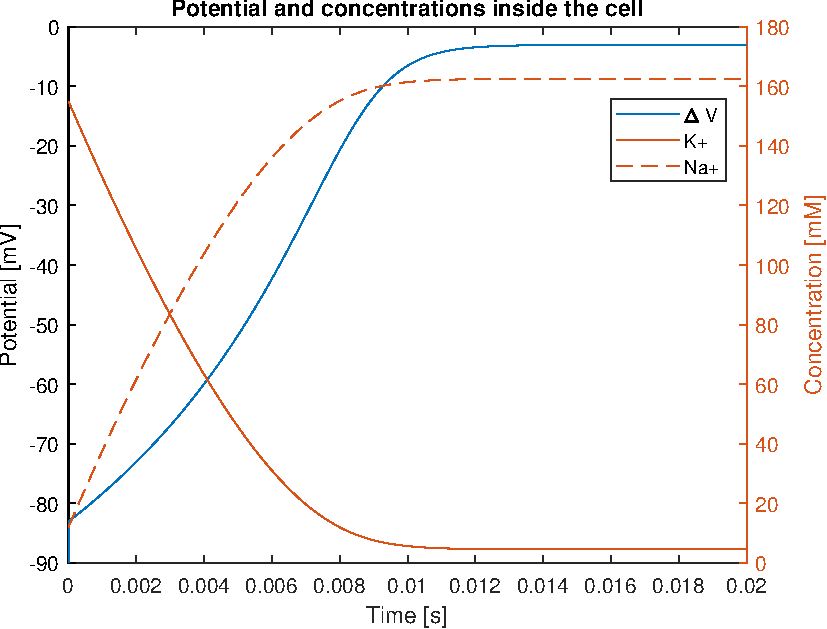
\includegraphics[width=0.65\textwidth]{potential_diffpot.pdf}
    \caption{Potential and concentrations as functions of time. Differential potential evolution.}
    \label{fig:potential_diffpot}
\end{figure}

\begin{figure}[H]
    \centering
    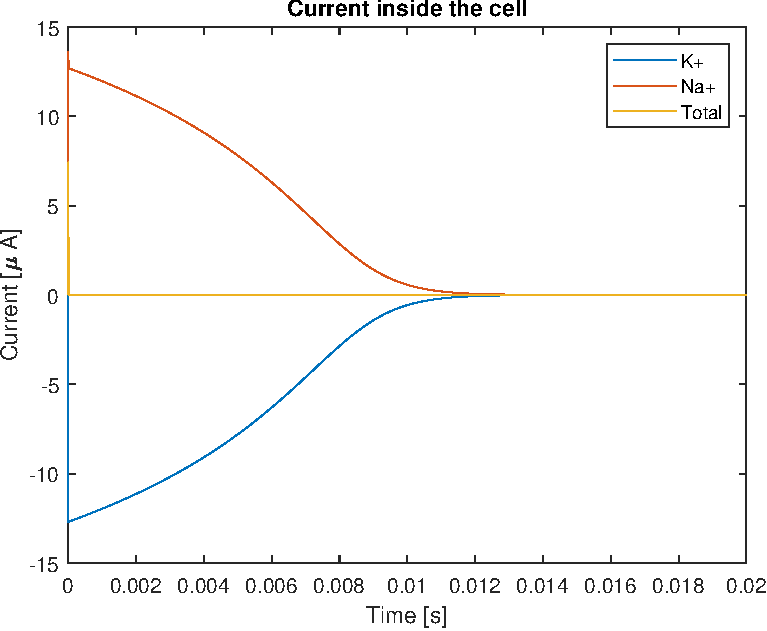
\includegraphics[width=0.65\textwidth]{current_diffpot.pdf}
    \caption{Current as functions of time. Differential potential evolution.}
    \label{fig:current_diffpot}
\end{figure}

As can be seen from the plots, at $t=0$ there is a positive current of sodium ions entering the cells and a negative one of potassium ions; this means that the internal concentration of sodium ions increase while the potassium one decrease. The process, as it's clear from the plots, reach an asymptotic equilibrium which is calculated to be:
\begin{gather*}
    C_i^K = 4.5 \si{mM}\\
    C_i^{Na} = 163 \si{mM}\\
    V = -3.0 \si{mV}
\end{gather*}

In this situation, fluxes are negligible: the cell have reach a static equilibrium. Observe that the found equilibrium concentration are similar to the extracellular ones, with a small difference due to the non-zero potential difference. 

\bigskip
Consider instead the presence of negative charges inside the cell, and eq. \eqref{eqn:potwithchar}. A second simulation has been performed considering the following update rules:
\begin{gather*}
    C_i(t+\Delta t) = C_i(t) + J(t) \frac{A}{V} \Delta t \\
    \Delta V(t+\Delta t) =  \frac{(z_KC_i^K(t+\Delta t) + z_{Na}C_i^{Na}(t+\Delta t))e\mathcal{V} + Q_-}{cA}
\end{gather*}

This second simulation method allow us to follow the temporal evolution of the total cell charge:

\begin{figure}[H]
    \centering
    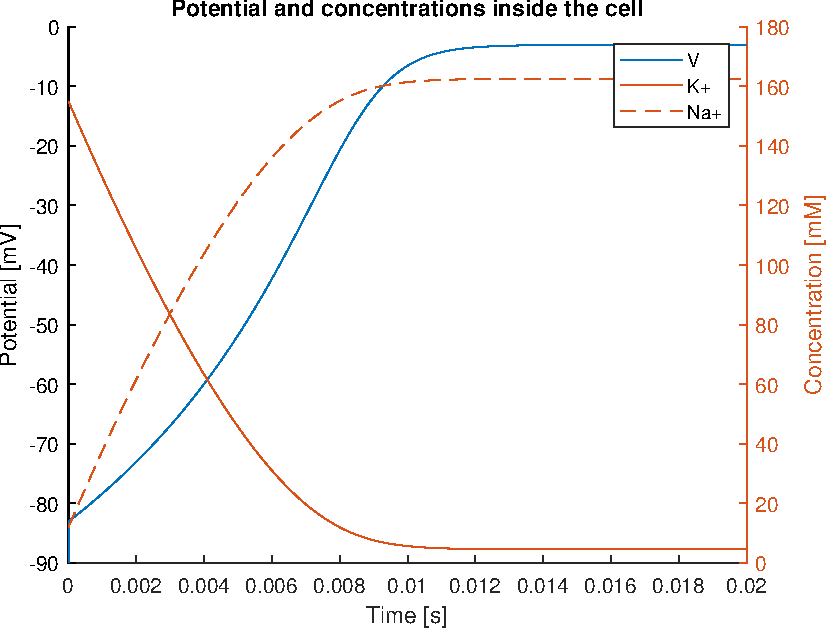
\includegraphics[width=0.65\textwidth]{potential_chargepot.pdf}
    \caption{Potential and concentrations as functions of time. Potential computed from charge.}
    \label{fig:potential_chargepot}
\end{figure}

\begin{figure}[H]
    \centering
    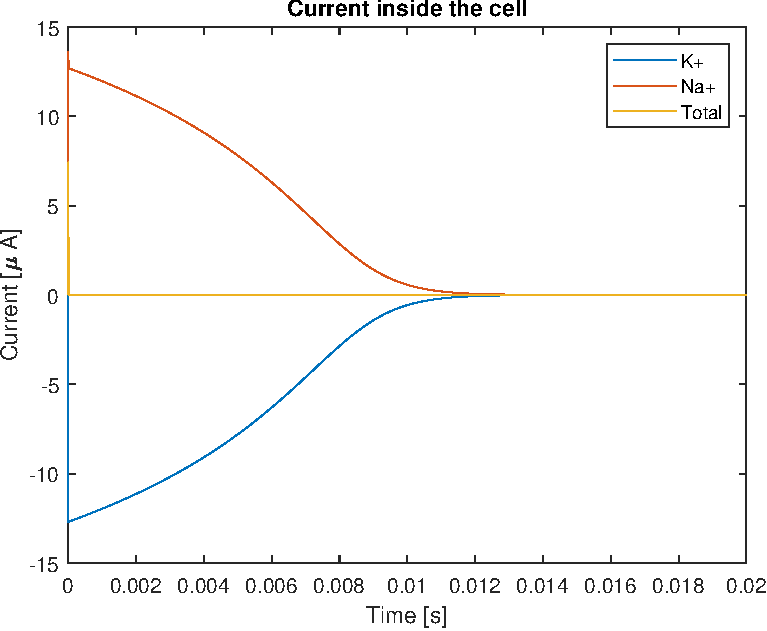
\includegraphics[width=0.65\textwidth]{current_chargepot.pdf}
    \caption{Current as functions of time. Potential computed from charge.}
    \label{fig:current_chargepot}
\end{figure}

\begin{figure}[H]
    \centering
    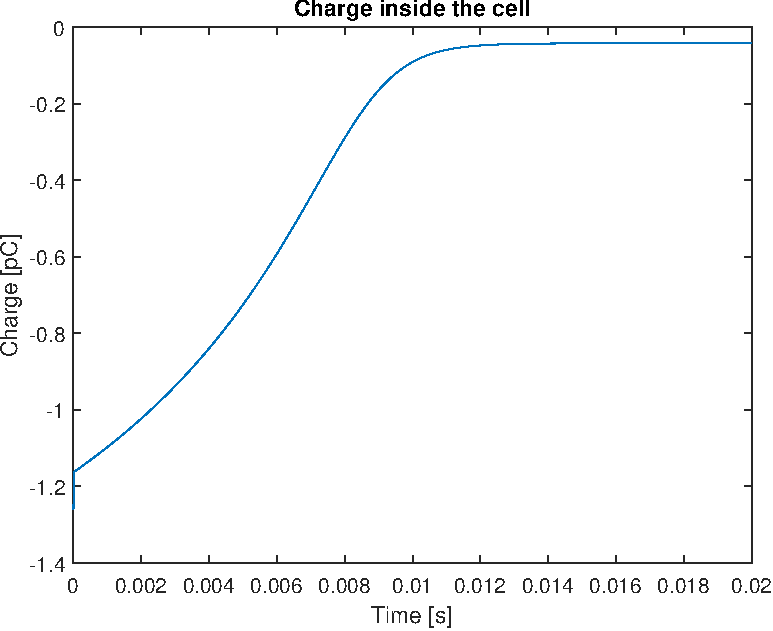
\includegraphics[width=0.65\textwidth]{charge_chargepot.pdf}
    \caption{Total charge as functions of time. Potential computed from charge.}
    \label{fig:charge_chargepot}
\end{figure}

As can be seen from the plot, the result of the time evolution is identical from the two methods, confirming us that they're both valid to simulate the system. Regarding the total charge, it's clear that the cell tend to the neutrality, reaching an equilibrium total charge (consider that the initial charge was $-1.26\si{pC}$) of:
\begin{align*}
    Q = -0.04 \si{pC}
\end{align*}

\section*{Conclusion}
In this paper, a non-excitable finite cell has been considered and the evolution of the concentration of sodium and potassium ions concentrations have been simulated. In particular, has been proven that if no active pumps are present the the cell go through a depolarization, reaching an equilibrium when the concentrations are similar to the extracellular ones. Moreover, two different methods for simulating the potential evolution have been tested, finding identical results. The second method, moreover, shows that the cell tends to the charge neutrality.

In the future, the simulation can be improved considering other ions, both positive and negative, which secondary contribute to cell depolarization. Moreover, \ch{Na+ / K+}-ATPase pumps can be added to study the energy needed to keep the correct physiological conditions.

\end{document}